\documentclass[runningheads]{llncs}
\usepackage{amsmath}
\usepackage{amssymb}
\usepackage{algorithm}
\usepackage[noend]{algpseudocode}
\usepackage{xspace}
\usepackage{mathtools}
\usepackage{graphicx}
\usepackage{array}
\usepackage{xcolor}
\usepackage{theorem}
\usepackage[T1]{fontenc}
\usepackage{hyperref}


\algrenewcommand\algorithmicprocedure{}
\algrenewcommand\algorithmicthen{}
\algrenewcommand\algorithmicdo{}

\newcommand{\fs}[1]{\fontsize{#1}{#1}\selectfont}
\newcommand{\fss}[2]{\fontsize{#1}{#2}\selectfont}
\newcommand{\sat}{SAT\xspace}
\newcommand{\code}[1]{\text{#1}}
\newcommand{\assertionTrail}{\trail}
\newcommand{\oneuip}{1-UIP\xspace}
\newcommand{\alluip}{all-UIP\xspace}
\newcommand{\LBD}{\text{LBD}\xspace}
\newcommand{\gap}{\text{gap}}
\newcommand{\tgap}{t_{\mathit{gap}}}
\newcommand{\ntries}{n_{\mathit{tries}}}
\newcommand{\nsuc}{n_{\mathit{succ}}}
\newcommand{\stablealluip}{\textit{stable-alluip}\xspace}
\newcommand{\tryuiplevel}{\textit{try-uip-level}\xspace}
\newcommand{\allUipPure}{\textit{pure-alluip}\xspace}
\newcommand{\allUipMin}{\textit{min-alluip}\xspace}
\newcommand{\allUipAct}{\textit{alluip-active}}
\newcommand{\allUipIn}{\textit{alluip-inclusive}}
\newcommand{\allUipEx}{\textit{alluip-exclusive}}
\newcommand{\MapleBase}{\textit{MapleCOMSPS-LRB}}
\newcommand{\MapleSeven}{\textit{MapleLCMDist}}
\newcommand{\MapleNine}{\textit{MapleLCMDiscChronoBT-DL-v3} }
\newcommand{\MapleEight}{\textit{MapleLCMDiscChronoBT}}
\newcommand{\MapleNineShort}{\textit{MapleCB-DL} }
\newcommand{\expSAT}{\textit{expMaple-CM-GCBumpOnlyLRB} }
\newcommand{\expSATShort}{\textit{expMaple} }
\newcommand{\cadical}{\textit{CaDiCaL}}
\newcommand{\defaultcadical}{\textit{CaDiCaL-default}}
\newcommand{\MapleIUIPPure}{\text{Maple-\allUipPure}}
\newcommand{\MapleIUIMin}{\text{Maple-\allUipMin}}
\newcommand{\MapleEightShort}{\textit{MapleCB}}
\newcommand{\Set}[2]{\{\,#1\mid#2\,\}}
\newcommand{\Array}[2]{[\,#1\mid#2\,]}
\newcommand{\trail}{\ensuremath{\mathcal{T}}}
\newcommand{\trailIdx}[1]{\ensuremath{\iota(#1)}}
\newcommand{\dlevel}[1]{\ensuremath{\mathit{decLvl}(#1)}}
\newcommand{\dlevels}{\ensuremath{\mathit{decLvls}}}
\newcommand{\var}{\text{var}}
\newcommand{\true}{\textsc{true}\xspace}
\newcommand{\false}{\textsc{false}\xspace}
\newcommand{\reason}[1]{\ensuremath{\mathit{reason}(#1)}}
\newcommand{\resolve}{\bowtie}
\renewcommand{\implies}{\rightarrow}
\newcommand{\ctry}{C_{\mathit{try}}}
\newcommand{\config}{\textit{config}}
\newcommand{\unmarked}{\textbf{unmarked}}
\newcommand{\mrk}{\textbf{mark}}
\setlength{\theorempreskipamount}{3pt}
\setlength{\theorempostskipamount}{3pt}

\newtheorem{Obs}{Observation}
\newtheorem{Cor}{Corollary}
\newtheorem{defn}{Definition}
\newtheorem{thm}{Theorem}

\newcommand{\whitebox}{\raisebox{.5ex}{\fbox{\hspace*{.2ex}}}}

%Comments
\newcommand{\nf}[1]{{\color{red}{#1}}}
\newcommand{\fb}[1]{{\color{blue}{#1}}}

\title{Clause Size Reduction with \alluip Learning}
\author{Nick Feng \and Fahiem Bacchus}
\authorrunning{N. Feng and F. Bacchus}
\institute{Department of Computer Science, University of Toronto, Canada, 
  \email{\{fengnick,fbacchus\}@cs.toronto.edu}}


\begin{document}
\maketitle              % typeset the header of the contribution
% 
\begin{abstract}
    Almost all CDCL \sat solvers use the \oneuip clause learning
    scheme for learning new clauses from conflicts, and our current
    understanding of \sat solving provides good reasons for using that
    scheme. In particular, the \oneuip scheme yields asserting
    clauses, and these asserting clauses have minimum \LBD among all
    possible asserting clauses. As a result of these advantages, other
    clause learning schemes, like $i$-UIP and \alluip, that were
    proposed in early work are not used in modern solvers. In this
    paper, we propose a new technique for exploiting the \alluip
    clause learning scheme.  Our technique is to employ \alluip
    learning under the constraint that the learnt clause's \LBD does
    not increase (over the minimum established by the \oneuip
    clause). Our method can learn clauses that are significantly
    smaller than the \oneuip clause while preserving the minimum
    \LBD. Unlike previous clause minimization methods, our technique
    is not limited to learning a sub-clause of the \oneuip clause. We
    show empirically that our method can improve the performance of
    state of the art solvers.
\end{abstract}

\section{Introduction}
Clause learning is an essential technique in \sat solvers. There is
good evidence to indicate that it is, in fact, the most important
technique used in modern \sat solvers
\cite{DBLP:conf/sat/KatebiSS11}. In early \sat research a number of
different clause learning techniques were proposed
\cite{DBLP:conf/iccad/ZhangMMM01,DBLP:conf/iccad/SilvaS96,DBLP:journals/tc/Marques-SilvaS99,DBLP:conf/aaai/BayardoS97}.
However, following the revolutionary performance improvements achieved
by the Chaff \sat solver, the field has converged on using the \oneuip
(first Unique Implication Point) scheme
\cite{DBLP:conf/iccad/ZhangMMM01} employed in Chaff
\cite{DBLP:conf/dac/MoskewiczMZZM01} (as well as other techniques
pioneered in the Chaff solver).\footnote{The idea of UIP clauses was
  first mentioned in \cite{DBLP:conf/iccad/SilvaS96}, and
  \oneuip clauses along with other UIP clauses were learnt and used in
  the earlier GRASP \sat solver.} Since then almost all \sat solvers
have employed the \oneuip clause learning scheme, along with clause
minimization \cite{DBLP:conf/sat/SorenssonB09}, as their primary
method for learning new clauses.

However, other clause learning schemes can be used in SAT solvers
without changes to the main data structures. Furthermore, advances in
our understanding allow us to better understand the potential
advantages and disadvantages of these alternate schemes. In this paper
we reexamine these previously proposed schemes with a focus on the
schemes described in \cite{DBLP:conf/iccad/ZhangMMM01}. Improved
understanding of \sat solvers, obtained from the last decade of
research, allows us to see that in their original form these
alternative clause learning schemes suffer significant disadvantages
over \oneuip clause learning.

One of the previously proposed schemes was the \alluip scheme
\cite{DBLP:conf/iccad/ZhangMMM01}. In this paper we propose a new way
to exploit the main ideas of this scheme that avoids its main
disadvantage which is that it can learn clauses with higher \LBD
scores. In particular, we propose to use a \alluip like clause
learning scheme to generate smaller learnt clauses which retain the
good properties of standard \oneuip clauses. Our method is related to,
but not the same as, various clause minimization methods that try to
remove redundant literals from the \oneuip clause yielding a clause that
is a subset of the \oneuip clause, e.g.,
\cite{DBLP:conf/sat/SorenssonB09,DBLP:conf/ijcai/LuoLXML17,DBLP:conf/sat/WieringaH13}.
Our method is orthogonal to clause minimization. In particular, our
approach can learn a clause that is not a subset of the \oneuip clause
but which still serves all of the same purposes as the \oneuip clause.
Clause minimization techniques can be applied on top of our method 
to remove redundant literals.

We present various versions of our method and show that these variants
are often capable of learning shorter clauses than the \oneuip scheme,
and that this can lead to useful performance gains in state of the art
\sat solvers.

\section{Clause Learning Framework}
We first provide some background and a framework for understanding
clause learning as typically used in CDCL \sat solvers. A
propositional formula $F$ expressed in Conjunctive Normal Form (CNF)
contains a set of variables $V$. A literal is a variable $v\in V$ or
its negation $\lnot v$. For a literal $\ell$ we let $\var(\ell)$
denote its underlying variable. A CNF consists of a conjunction of
clauses, each of which is a disjunction of literals. We often view a
clause as being a set of literals and employ set notation, e.g.,
$\ell\in C$ and $C'\subset C$. 

Two clauses $C_1$ and $C_2$ can be \emph{resolved} when they contain
\emph{conflicting} literals $\ell\in C_1$ and $\lnot \ell \in
C_2$. Their resolvent $C_1 \resolve C_2$ is the new clause
$(C_1 \cup C_2) - \{\ell, \lnot \ell\}$. The resolvent will be a
tautology (i.e., a clause containing a literal $x$ and its negation
$\lnot x$) if $C_1$ and $C_2$ contain more than one pair of
conflicting literals.

We assume the reader is familiar with the operations of CDCL \sat
solvers, and the main data structures used in such solvers. A good
source for this background is \cite{DBLP:series/faia/SilvaLM09}.

\vspace*{3pt}\noindent\textit{The Trail.}
CDCL \sat solvers maintain a \textbf{trail}, $\trail$, which is a
\textit{non-contradictory, non-redundant sequence of literals} that
have been assigned \true by the solver; i.e.
$\ell\in\trail \implies \lnot\ell \not\in\trail$, and $\trail$
contains no duplicates. Newly assigned literals are added to the end
of the trail, and on backtrack literals are removed from the end of
the trail and unassigned.  If literal $\ell$ is on the trail let
$\trailIdx{\ell}$ denote its index on the trail, i.e,
$\trail[\trailIdx{\ell}] = \ell$. For convenience, we also let
$\trailIdx{\ell} = \trailIdx{\lnot \ell} = \trailIdx{\var(\ell)}$ even
though neither $\lnot \ell$ nor $\var(\ell)$ are actually on
$\trail$. If $x$ and $y$ are both on the trail and
$\trailIdx{x} < \trailIdx{y}$ we say that \textit{$x$ appears before
  $y$ on the trail}. 

Two types of true literals appear on the trail: \emph{decision
  literals} that have been assumed to be true by the solver, and
\emph{unit propagated literals} that are \emph{forced to be true}
because they are the sole remaining unfalsified literal of a
clause. Each literal $\ell\in\trail$ has a decision level
$\dlevel{\ell}$. Let $k$ be the number of decision literals appearing
before $\ell$ on the trail. When $\ell$ is a unit propagated literal
$\dlevel{\ell}=k$, and when $\ell$ is a decision literal
$\dlevel{\ell}=k+1$. For example, $\dlevel{d}=1$ for the first
decision literal $d\in\trail$, and $\dlevel{\ell}=0$ for all literals
$\ell$ appearing before $d$ on the trail.  The set of literals on
$\trail$ that have the same decision level forms a contiguous
subsequence of $\trail$ that starts with a decision literal $d_i$ and
ends just before the next decision literal $d_{i+1}$. If
$\dlevel{d_i} = i$ we call this subsequence of $\trail$ the
\textit{$i$-th decision level}.

Each literal $\ell\in\trail$ also has a clausal reason
$\reason{\ell}$. If $\ell$ is a unit propagated literal,
$\reason{\ell}$ is a clause of the formula such that
$\ell \in \reason{\ell}$ and
$\forall x \in \reason{\ell}.\, x\neq \ell \implies \bigl(\lnot x \in
\trail \land \trailIdx{\lnot x} < \trailIdx{\ell}\bigr)$. That is,
$\reason{\ell}$ is a clause that has become unit implying $\ell$ due
to the literals on the trail above $\ell$. If $\ell$ is a decision
literal then $\reason{\ell} = \varnothing$.

In most \sat solvers, clause learning is initiated as soon as a clause
is falsified by $\trail$. In this paper we will be concerned with the
subsequent clause learning process which uses $\trail$ to derive a new
clause. We will try to make as few assumptions about how $\trail$ is
managed by the \sat solver as possible. One assumption we will make is
that $\trail$ \emph{remains intact during clause learning} and is only
changed after the new clause is learnt (by backtracking). 

Say that $\trail$ falsifies a clause $C_I$, and that the last decision
literal $d_k$ in $\trail$ has decision level $k$. Consider
$\trail_{k-1}$ the prefix of $\trail$ above the last decision level,
i.e., the sequence of literals
$\trail[0]$---$\trail[\trailIdx{d_k}-1]$. We will assume that
$\trail_{k-1}$ is \textbf{unit propagation complete}, although the
full trail $\trail$ might not be. This means that (a) no clause was
falsified by $\trail_{k-1}$. And (b) if $C_u$ is a clause containing
the literal $x$ and all literals in $C_u$ except for $x$ are falsified
by $\trail_{k-1}$, then $x\in \trail_{k-1}$ and
$\dlevel{x} \leq\max\{\dlevel{y} | y\in C_u \land y\neq x\}$. This
means that if $x$ appears in a clause made unit it must have been
added to the trail, and added at or before decision level the clause
became unit. Note that more than one clause might be made unit by
$\trail$ forcing $x$, or $x$ might be set as a decision before being
forced. This condition ensures that $x$ appears in $\trail$ at or
before the first decision level it is forced by any clause.

Any clause falsified by $\trail$ is called a \textbf{conflict}. When a
conflict is found, the final level of the trail, $k$, need not be unit
propagation complete as the solver typically stops propagation as soon
as it finds a conflict. This means that (a) other clauses might be
falsified by $\trail$ besides the conflict found, and (b) other
literals might be unit implied by $\trail$ but not added to $\trail$.

\begin{defn}[Trail Resolvent]
    A trail resolvent is a clause arising from resolving a conflict
    against the reason clause of some literal $\ell \in \trail$. Every
    trail resolvent is also a conflict.
\end{defn}

The following things can be noted about trail resolvents: (1) trail
resolvents are never tautological, as the polarity of all literals in
$\reason{\ell}$ other than $\ell$ must agree with the polarity of all
literals in the conflict (they are all falsified by $\trail$); (2) one
polarity of the variable $\var(\ell)$ resolved on must be a unit
propagated literal whose negation appears in the conflict; and (3) any
variable in the conflict that is unit propagated in $\trail$ can be
resolved upon (the variable must appear in different polarities in the
conflict and in $\trail$).

\begin{defn}[Trail Resolution]
    A trail resolution is a sequence of trail resolvents applied to an
    initial conflict $C_I$ yielding a new conflict $C_L$.  A trail
    resolution is \textbf{ordered} if the sequence of variables $v_1$,
    \dots, $v_m$ resolved have strictly decreasing trail indices:
    $\trailIdx{v_{i+1}} < \trailIdx{v_i}$ ($1\leq i < m$). (Note that
    this implies that no variable is resolved on more than once).
\end{defn}

Ordered trail resolutions resolve unit propagated literals from the
end of the trail to the beginning. W.l.o.g we can require that all trail
resolutions be ordered.

\begin{Obs}
    \label{obs:ordered}
    If the unordered trail resolution $U$ yields the conflict clause
    $C_L$ from an initial conflict $C_I$, then there exists an ordered
    trail resolution $O$ that yields a conflict clause $C'_L$ such
    that $C'_L\subseteq C_L$.
\end{Obs}
\noindent
\textbf{Proof.} Let $U$ be the sequence of clauses $C_I = C_0$, $C_1$,
$\ldots$, $C_m= C_L$ obtained by resolving on the sequence of
variables $v_1$, $\ldots$, $v_m$ whose corresponding literals on
$\trail$ are $l_1$, $\ldots$, $l_m$. Reordering these resolution steps
so that the variables are resolved in order of decreasing trail index
and removing duplicates yields an ordered trail resolution $O$ with
the desired properties. Since no reason clause contains literals with
higher trail indices, $O$ must be a valid trail resolution if $U$
was, and furthermore $O$ yields the clause
$C'_L = \bigcup_{i=1}^m \reason{l_i} - \{l_1, \lnot l_1, \ldots, l_m,
\lnot l_m\}$. Since $U$ resolves on the same variables (in a different
order) using the same reason clauses we must have $C'_L\subseteq
C_L$. It can, however, be the case that $C'_L$ is proper subset of
$C_L$: if $l_i$ is resolved away it might be reintroduced when
resolving on $l_{i+1}$ if $\trailIdx{l_{i+1}}  > \trailIdx{l_i}$.
\whitebox

The relevance of trail resolutions is that all proposed clause
learning schemes we are aware of use trail resolutions to produce
learnt clauses. Furthermore, the commonly used technique for clause
minimization \cite{DBLP:conf/sat/SorenssonB09} is also equivalent to a
trail resolution that yields the minimized clause from the
un-minimized clause. Interestingly, it is standard in \sat solver
implementations to perform resolution going backwards along the
trail. That is, these implementations are typically using ordered
trail resolutions. Observation~\ref{obs:ordered} shows that this is
correct.

Ordered trail resolutions are a special case of \textit{trivial
  resolutions} \cite{DBLP:journals/jair/BeameKS04}. Trail resolutions
are specific to the trail data structure typically used in \sat
solvers. If $\trail$ falsifies a clause at its last decision level,
then its associated implication graph
\cite{DBLP:journals/tc/Marques-SilvaS99} contains a conflict
node. Cuts in the implication graph that separate the conflict from
the rest of the graph correspond to conflict clauses
\cite{DBLP:journals/jair/BeameKS04}. It is not difficult to see that
the proof Proposition~4 of \cite{DBLP:journals/jair/BeameKS04} applies
also to trail resolutions. This means that \textit{any conflict clause
  in the trail's implication graph can be derived using a trail
  resolution.}

\subsection{Some Alternate Clause Learning Schemes}
A number of different clause learning schemes for generating a new
learnt clause from the initial conflict have been presented in prior
work, e.g.,
\cite{DBLP:conf/iccad/ZhangMMM01,DBLP:conf/iccad/SilvaS96,DBLP:journals/tc/Marques-SilvaS99,DBLP:conf/aaai/BayardoS97}.
Figure~\ref{fig:cl_schemes} gives a specification of some of these
methods: (a) the all-decision scheme which resolves away all implied
literals leaving a learnt clause over only decision literals; (c) the
\oneuip scheme which resolves away literals from the deepest decision
level leaving a learnt clause with a single literal at the deepest
level; (d) the \alluip scheme which resolves away literals from each
decision level leaving a learnt clause with a single literal at each
decision level; and (e) the $i$-UIP scheme which resolves away
literals from the $i$ deepest decision levels leaving a learnt clause
with a single literal at its $i$ deepest decision levels. It should be
noted that when resolving away literals at decision level $i$, new
literals at decision levels less than $i$ might be introduced into the
clause. Hence, it is important in the $i$-UIP and \alluip schemes to
use ordered trail resolutions.

Both the all-decision and \alluip schemes yield a clause with only one
literal at each decision level, and the \alluip clause will be no
larger that the all-decision clause. Furthermore, it is known
\cite{DBLP:journals/tc/Marques-SilvaS99} that once we reduce the
number of literals at a decision level $d$ to one, we could continue
performing resolutions and later achieve a different single literal at
the level $d$. In particular, a decision level might contain more than
one unique implication point, and in some contexts the term all-UIP is
used to refer to all the unique implication points that exist in a
particular decision level \cite{DBLP:conf/sat/SabharwalSS12} rather
than the \alluip clause learning scheme as is used here. The
algorithms given in Figure~\ref{fig:cl_schemes} stop at the first UIP
of a level, except for the all-decision schemes with stops at the last
UIP of each level.

{\setlength{\textfloatsep}{-10pt plus 1.0pt minus 2.0pt}
\begin{figure}[t!]
{\fss{8pt}{9pt}
\setlength{\tabcolsep}{0.02em}
\begin{tabular}[t]{|c|c|c|}
  \cline{1-1}\cline{3-3}
  \begin{minipage}[t]{0.5\textwidth}
    \textbf{(a) All Decision Clause\rule{0pt}{1.1\topskip}}
    \begin{algorithmic}[0]
        \State \hspace*{-.7em}\textbf{all-decision}($C_I$)
        \State $C\gets C_I$
        \While{$\{l\,|\, l\in C \land\reason{l} \neq\varnothing\} \neq \emptyset$}
        \State \begin{tabular}{ll}
                 $\ell \gets \mbox{}$ & literal with highest trail index in\\
                                      & $\{l\,|\, l\in C \land\reason{l} \neq\varnothing\}$
               \end{tabular}
        \State $C \gets C\resolve \reason{\lnot \ell}$
        \EndWhile
        \State \textbf{return} $C$
    \end{algorithmic}
  \end{minipage}
  & &
  \begin{minipage}[t]{0.5\textwidth}
      \textbf{(b) Make level $i$ contain a single literal\rule{0pt}{1.1\topskip}}
      \begin{algorithmic}[0]
          \State \hspace*{-.7em} \textbf{UIP-level}($C$, $i$)
          \While{$\left|\left\{\ell \left| \begin{array}{l}\ell \in C\\
                                           \mbox{}\land \reason{l} \neq \varnothing \\
                                           \mbox{}\land \dlevel{l} = i\end{array}\right.\right\}\right| > 1$}
          \State \begin{tabular}{ll}
                   $l \gets \mbox{}$ & literal with highest trail index in\\
                                        & $\left\{\ell \left| \begin{array}{l}\ell \in C
                                          \land \reason{l} \neq \varnothing \\
                                          \mbox{}\land \dlevel{l} = i\end{array}\right.\right\}$
                 \end{tabular}
          \State $C \gets C\resolve \reason{\lnot l}$
          \EndWhile
          \State \textbf{return} $C$\strut
      \end{algorithmic}
  \end{minipage}
  \\\cline{1-1}\cline{3-3}
   \multicolumn{1}{c}{\vspace*{-7pt}}\\\cline{1-1}\cline{3-3}
  \begin{minipage}[t]{0.5\textwidth}
    \begin{minipage}{\textwidth}
        \textbf{(c) First UIP Clause \rule{0pt}{1.1\topskip}}
        \begin{algorithmic}[0]
            \State \hspace*{-.7em}\textbf{\oneuip}($C_I$)
            \State $i\gets \max\{\dlevel{l}\, |\, l \in C_I\}$
            \State \textbf{return} \textbf{UIP-level}($C_I$, i)
        \end{algorithmic}
        \vspace*{5pt}
    \end{minipage}\\[5pt]
    \hspace*{-.6pt}\rule{1.005\textwidth}{.4pt}\\[5pt]
    \begin{minipage}{\textwidth}
        \textbf{(d) \alluip Clause \rule{0pt}{1.1\topskip}}
        \begin{algorithmic}[0]
          \State \hspace*{-.7em}\textbf{\alluip}($C_I$, $i$)
          \State $i = \bigl|\{\dlevel{l} \,|\, l \in \trail\}\bigl|$
          \State \Comment{{\fs{7pt}$i$ is large enough to ensure all levels are UIP}}
          \State \textbf{return} \textbf{$i$-UIP}(C, i)

      \end{algorithmic}
      \end{minipage}
  \end{minipage}
 & &
  \begin{minipage}[t]{0.5\textwidth}
      \vspace*{-20pt}
      \textbf{(e) $i$-UIP Clause}
      \begin{algorithmic}[0]
          \State \hspace*{-.7em}\textbf{$i$-UIP}($C_I$, $i$)
          \State $C\gets C_I$
          \State $d\gets \max\{\dlevel{l}\,|\, l \in C\}$
          \For{($j \gets 1$; $j\leq i$; $j\gets j+1$)}
          \State \textbf{if} ($d = \varnothing$): \textbf{break}
          \State $C\gets\mbox{}$ \textbf{UIP-level(C, d)}
          \State $d\gets \max\left\{\dlevel{l} \left|\begin{array}{l}l\in C \\ \mbox{} \land \dlevel{l}<d
                                                  \end{array}\right.\right\}$
          \EndFor
          \State \textbf{return} $C$\strut
      \end{algorithmic}
      \vspace*{3pt}
      \textit{Maximum of an empty set is $\varnothing$ \strut}
  \end{minipage}
\\\cline{1-1}\cline{3-3}
\end{tabular}
}
\vspace*{-5pt}
\caption{Some different clause learning schemes. All use the
      current trail $\trail$ and take as input an initial clause $C_I$
      falsified by $\trail$ at its deepest level.\label{fig:cl_schemes}}
\end{figure}
}
 %   \floatstyle{boxed}
 %   \restylefloat{figure}


\subsection{Asserting Clauses and \LBD---Reasons to Prefer \oneuip
  Clauses}
An \textbf{asserting clause} \cite{DBLP:journals/ai/PipatsrisawatD11}
is a conflict clause $C_L$ that has exactly one literal $\ell$ at its
deepest level, i.e.,
$\forall x\in C_L. \dlevel{x} \leq \dlevel{\ell} \land (\dlevel{x} =
\dlevel{\ell} \implies x = \ell$). All of the clause learning schemes in
Figure~\ref{fig:cl_schemes} produced learnt clauses that are asserting.

The main advantage of asserting clauses is that they are 1-Empowering
\cite{DBLP:journals/ai/PipatsrisawatD11}, i.e., they allow unit
propagation to derive a new forced literal. Hence, asserting clauses
can be used to guide backtracking---the solver can backtrack from the
current deepest level to the point the learnt clause first becomes
unit, and then use the learnt clause to add a new unit implicant to
the trail. Since all but the deepest level was unit propagation
complete, this means that the asserting clause must be a brand new
clause; otherwise that unit implication would already have been
made. On the other hand, if the learnt clause $C_L$ is not asserting
then it could be that it is a duplicate of another clause already in
the formula.

\begin{example}
    Suppose that $a$ is a unit propagated literal and $d$ is a
    decision literal with $\dlevel{d}>\dlevel{a}$. Let the sequence of
    clauses watched by $\lnot d$ be $(\lnot d$, $x$, $\lnot a)$,
    $(\lnot d$, $y$, $\lnot x$, $\lnot a)$, $(\lnot d$, $\lnot y$,
    $\lnot x$, $\lnot a)$, $(\lnot d$, $\lnot x$, $\lnot a)$. When $d$
    is unit propagated the clauses on $\lnot d$'s watch list will be
    checked in this order.

    Hence, unit propagation of $d$ will extend the trail by first
    adding the unit propagated literal $x$ (with $\reason{x}=(x$,
    $\lnot d$, $\lnot a)$) and then the unit propagated literal $y$
    (with $\reason{y}=(y$, $\lnot x$, $\lnot a$, $\lnot d)$). Now the
    third clause on $\lnot d$'s watch list, $(\lnot d$, $\lnot y$,
    $\lnot x$, $\lnot a)$ is detected to be a conflict. 

    Clause learning can now be initiated from conflict $C_I=(\lnot d$,
    $\lnot y$, $\lnot x$, $\lnot a)$. This clause has 3 literals at
    level $\dlevel{d}=10$. If we stop clause learning before reaching
    an asserting clause, then it is possible to simply resolve $C_I$
    with $\reason{y}$ to obtain the learnt clause $C_L = (\lnot d$,
    $\lnot x$, $\lnot a)$. However, this non-asserting learnt clause
    is a duplicate of the fourth clause on $\lnot d$'s watch list
    which is already in the formula.\footnote{In this example, the
      fourth clause on $\lnot d$'s watch list subsumes the third
      clause. But it is not difficult to construct more elaborate
      examples where there are no subsumed clauses and we still obtain
      learnt clauses that are duplicates of clauses already in the
      formula.}  This issue can arise whenever $C_L$ contains two or
    more literals at the deepest level (i.e., whenever $C_L$ is not
    asserting). In such cases $C_L$ might be a clause already in the
    formula with its two watches not yet fully unit propagated (and
    thus $C_L$ is not detected by the \sat solver to be a conflict)
    since propagation is typically stopped as soon as a conflict is
    detected.

\end{example}


The \LBD of the learnt clause $C_L$ is the number of different decision
levels in it:
$\LBD(C_L)=\left|\big\{\dlevel{l}\,|\,l \in C_L\big\}\right|$
\cite{DBLP:conf/ijcai/AudemardS09}. Empirically \LBD is a successful
predictor of clause usefulness: clauses with lower \LBD tend to be more
useful. As noted in \cite{DBLP:conf/ijcai/AudemardS09}, from the
initial falsified clause $C_I$ the \oneuip scheme will produce a clause
$C_L$ whose \LBD is minimum among all asserting clauses that can be
learnt from $C_I$. If $C'$ is a trail resolvent of $C$ and a reason
clause $\reason{l}$, then $\LBD(C') \geq \LBD(C)$ since $\reason{l}$
must contain at least one other literal with the same decision level
as $l$ and might contain literals with decision levels not in
$C$. That is, the each trail resolution step might increase the \LBD
of the learnt clause and can never decrease the \LBD. Hence, the \oneuip
scheme yields an asserting clause with minimum \LBD as it performs the
minimum number of trail resolutions required to generate an asserting
clause.

The other schemes must perform more trail resolutions. In fact, all of
these schemes (all-decision, all-UIP, i-UIP) use trail resolutions in
which the \oneuip clause appears. That is, they all must first
generate the \oneuip clause and then continue with further trail
resolution steps. These extra resolution steps can introduce many
addition decision levels into the final clause. Hence, these schemes
learn clauses with \LBD at least as large as the \oneuip clauses.

Putting these two observations together we see that the \oneuip scheme
produces asserting clauses with lowest possible \LBD. This is a
compelling reasons for using this scheme. Hence, it is not surprising
that modern \sat solvers almost exclusively use \oneuip clause
learning.\footnote{Knuth in his sat13 CDCL solver \cite{Knuth:Sat13}
  uses an all-decision clause when the \oneuip clause is too large. In
  this context an \alluip clause could also be used as it would be no
  larger than the all decision clause.}

\section{Using \alluip Clause Learning}
\label{sec:i-uip}
Although learning clauses with low \LBD has been shown empirically to
be more important in \sat solving than learning short clauses
\cite{DBLP:conf/ijcai/AudemardS09}, clause size is still
important. Smaller clauses consume less memory and help to decrease
the size of future learnt clauses. They are also semantically stronger
than longer clauses.

The \alluip scheme will tend to produce small clauses since the
clauses contain at most one literal per decision level. However, the
\alluip clause can have much higher \LBD. Since $\LBD$ is more
important than size, our approach is to use \alluip learning when, and
only when, it succeeds in reducing the size of the clause
\emph{without increasing its \LBD}. The \alluip scheme first computes
the \oneuip clause when it reduces the deepest level to a single UIP
literal. It then proceeds to reduce the shallower levels (see
\alluip's for loop in Figure~\ref{fig:cl_schemes}). So our approach
will start with the \oneuip clause and then try to apply \alluip
learning to reduce other levels to single literals. As noted above,
clause minimization is orthogonal to our approach, so we also first
apply standard clause minimization \cite{DBLP:conf/sat/SorenssonB09}
to the \oneuip clause. That is, our algorithm $\stablealluip$
(Algorithm~\ref{alg:i-uip}), starts with the clause that most \sat
solvers learn from a conflict, a minimized \oneuip clause.

\begin{algorithm}[!t]
\caption{\stablealluip}\label{alg:i-uip}
\fss{9pt}{10pt}
\begin{algorithmic}[1]
    \Require $C_1$ is minimized \oneuip clause
    \Require \config{} a set of configuration parameters to give different versions \stablealluip.
    \Require $\tgap\geq 0$ is a global parameter, $\ntries$ and $\nsuc$ are used to
         dynamically adjust $\tgap$

    \Procedure{\stablealluip}{$C_1, \assertionTrail$}
    \State \textbf{if} ($|C_1| - \LBD(C_1) < \tgap$) \textbf{return} $C_1$\label{ln:control} 
    \State $\ntries$++\label{ln:try} 
    \State $C_i \gets C_1$
    \State $\dlevels \gets\mbox{}$ decision levels in $C_1$ in descending order\label{ln:init_loop}
        \Comment{These never change}
    \For{($i=1$; $i < |\dlevels|$; $i$++)}\label{ln:begin_level_loop}
         \Comment{skip the deepest level $\dlevels[0]$}
        \State $C_i\gets\mbox{}$\tryuiplevel($C_i$, $\dlevels[i]$) 
            \Comment{Try to reduce this level to UIP}
        \If{$\bigl|\{\ell\,|\,\ell \in C_i \land \dlevel{\ell} \geq
            \dlevels[i]\}\bigr| + (|\dlevels| - (i+1)) \geq
            |C_1|$}\label{ln:earlyTerminate}
            \State \textbf{return} $C_1$ 
                \Comment{can't generate smaller clause}\label{ln:end_level_loop}
        \EndIf
   \EndFor
   \If{$\mathbf{\allUipPure} \in \config$}
       \State $C_i \gets \mathbf{minimize}(C_i)$\label{ln:puremin}
   \EndIf
   \If{$\bigl(|C_i| < |C_1| \land 
       \mathbf{\allUipAct}\in\config\implies(\code{AvgVarAct}(C_i) > \code{AvgVarAct}(C_1))$
      \label{ln:activity}}
        \State $\nsuc$++, \textbf{return} $C_i$  \label{ln:returnmin}\label{ln:suc}
        \Comment{$C_i$ is smaller than the input clause}
   \Else \State \textbf{return} $C_1$
   \EndIf
\EndProcedure
\Statex 
\Procedure{\tryuiplevel}{$C_i$, $i$}
    \Comment{Do not add new decision levels}
    \State $\ctry = C_i$
    \State $L_i = \left\{\ell \left| \ell \in \ctry 
                         \land \dlevel{l} = i\right.\right\}$\label{ln:litsati1}
    \While{$|L_i| > 1$}
        \State $p \gets\mbox{}$ \textbf{remove} lit with the highest trail index from $L_i$ 
        \If{($\exists q \in \reason{\lnot p}.\, \dlevel{q} \not \in \mathit{decLvls}$)}\label{ln:newdlevel}
        \Comment{Would add new decision levels}
             \If{($\mathbf{\allUipPure}\in \config$)}
                 \State \textbf{return} $C_i$ \Comment{Abort, can't UIP this level}
             \ElsIf{($\mathbf{\allUipMin}\in\config$)}
                 \State \textbf{continue} \Comment{Don't try to resolve away $p$}
             \EndIf
        \Else\label{ln:nonewdlevel}
            \State $\ctry \gets \ctry \resolve \reason{\lnot p}$
            \State $L_i = L_i \cup \{\ell\,|\, 
                                     \ell\in\reason{\lnot p} \land \ell\neq \lnot p \land \dlevel{\ell} = i
                                    \}$\label{ln:litsati2}
        \EndIf
     \EndWhile
    \State \textbf{return} $\ctry$
\EndProcedure
\end{algorithmic}
\end{algorithm}


Algorithm~\ref{alg:i-uip} tries to compute a clause shorter than the
inputted \oneuip clause $C_1$. If a clause shorter than $C_1$ cannot
be computed the routine returns $C_1$ unchanged. Line~\ref{ln:control}
uses the parameter $\tgap$ to predict if Alg.~\ref{alg:i-uip} will be
successful in producing a shorter clause. This predication is
described below. If the prediction is negative $C_1$ is immediately
returned and Alg.~\ref{alg:i-uip} is not attempted. Otherwise, a copy
of $C_1$ is made in $C_i$ and $\ntries$, which counts the number of
times Alg.~\ref{alg:i-uip} is attempted, is incremented.

Then the decision levels of $C_1$ are computed and stored in
$\dlevels$ in order from largest to lowest. The for loop of
lines~\ref{ln:begin_level_loop}--\ref{ln:end_level_loop} is then
executed for each decision level $\dlevels[i]$. In the loop the
subroutine \tryuiplevel tries to reduce the set of literals at
$\dlevels[i]$ down to a single UIP literal using a sequence of trail
resolutions. Since $C_1$ is a \oneuip clause $\dlevels[0]$ (the
deepest level) already contains only one literal, so we can start at
$i=1$.

After the call to \tryuiplevel a check (line~\ref{ln:earlyTerminate})
is made to see if we can abort further processing. At this point the
algorithm has finished processing levels $\dlevels[0]$--$\dlevels[i]$
so the literals at those levels will not change. Furthermore, we know that
the best that can be done from this point on is to reduce the
remaining $|\dlevels| - (i+1)$ levels down to a single literal
each. Hence, adding these two numbers gives a lower bound on the size
of the final computed clause. If that lower bound is as large as the
size of the initial \oneuip clause we can terminate and return the initial
\oneuip clause.

After processing all decision levels, if \tryuiplevel is using the
\allUipPure configuration, additional reduction in the clause size
might be achieved by an another round of clause minimization
(line~\ref{ln:puremin}). Finally, if the newly computed clause $C_i$
is smaller that the input clause $C_1$ it is returned. Otherwise the
original clause $C_1$ is returned. Additionally, if the configuration
$\allUipAct$, described in Section~\ref{sec:active}, is being used,
then we also require that the average activity level of the new clause
$C_i$ be larger than $C_1$ before we can return the new clause $C_i$.

\tryuiplevel($C_i$, $i$) attempts to resolve away the literals at
decision level $i$ in the clause $C_i$, i.e., those in the set $L_i$
(line~\ref{ln:litsati1}), in order of decreasing trail index, until
only one literal at level $i$ remains. If the resolution step will not
introduce any new decision levels (line~\ref{ln:nonewdlevel}), it is
performed updating $\ctry$. In addition, all new literals added to
$\ctry$ at level $i$ are added to $L_i$. 

On the other hand, if the resolution step would introduce new decision
levels (line~\ref{ln:newdlevel}) then there are two options.  The
first option we call $\allUipPure$. With $\allUipPure$ we abort our
attempt to UIP this level and return the clause with level $i$
unchanged. In the second option, called $\allUipMin$, we continue
without performing the resolution, keeping the current literal $p$ in
$\ctry$. $\allUipMin$ then continues to try to resolve away the other
literals in $L_i$ (note that $p$ is no longer in $L_i$) until $L_i$ is
reduced to a single literal. Hence, $\allUipMin$ can leave multiple
literals at level $i$---all of those with reasons containing new
levels along with one other.\footnote{Since the sole remaining literal
  $u\in L_i$ is at a lower trail index than all of the other literals
  there is no point in trying to resolve away $u$---either it will be
  the decision literal for level $i$ having no reason, or its reason
  will contain at least one other literal at level $i$.} Observe that
the number of literals at level $i$ can not be increased after
processing it with \allUipPure. \allUipMin can, however, potentially
increase the number of literals at level $i$. In resolving away a
literal $l$ at level $i$, more literals might be introduced into level
$i$, and some of these might not be removable by \allUipMin if their
reasons contain new levels. However, both \allUipPure and \allUipMin
can increase the number of literals at levels less that $i$ as new
literals can be introduced into those levels when the literals at
level $i$ are resolved away. These added literals at the lower levels
might not be removable from the clause, and thus both methods 
can yield a longer clause than the input \oneuip clause.

After trying to UIP each level the clause $C_i$ is obtained. If we
were using $\allUipPure$ we can once again apply recursive clause
minimization (line~\ref{ln:puremin})
\cite{DBLP:conf/sat/SorenssonB09}, but this would be useless when
using $\allUipMin$ as all but one literal of each level introduces a
new level and thus cannot be recursively removed.\footnote{Other more
  powerful minimization techniques could still be applied.}


\noindent\textbf{$\tgap$}:\,\,
$\stablealluip$ can produce significantly smaller clauses. However,
when it does not yield a smaller clause, the cost of the additional
resolution steps can hurt the solver's performance. Since resolution
cannot reduce a clause's $\LBD$, the maximum size reduction obtainable
from $\stablealluip$ is the difference between the \oneuip clause's
size and its $\LBD$: $\gap(C_1) = |C_1| - \LBD(C_1)$. When $\gap(C_1)$
is small, applying $\stablealluip$ is unlikely to be cost
effective. Our approach is to dynamically set a threshold on
$\gap(C_1)$, $\tgap$, such that when $\gap(C_1) < \tgap$ we do not
attempt to reduce the clause (line~\ref{ln:control}). Initially,
$\tgap = 0$, and we count the number of times $\stablealluip$ is
attempted ($\ntries$) and the number of times it successfully yields a
shorter clause ($\nsuc$) (line~\ref{ln:try} and \ref{ln:suc}). On
every restart if the success rate since the last restart is greater
than 80\% (less than 80\%), we decrease (increase) $\tgap$ by one
not allowing it to become negative.

%\vspace*{-3pt}
\begin{example}
    Consider the trail $\assertionTrail = \ldots$, $\ell_1$, $a_2$, $b_2$,
    $c_2$,$d_2$, $\ldots$, $\ldots$, $e_5$, $f_5$, $g_5$,
    $h_6$, $i_6$, $j_6$, $k_6$, $\ldots$, $m_{10}$,
    $\ldots$ where the subscript indicates the decision level of each
    literal and the literals are in order of increasing trail
    index. 
    \[\fss{9pt}{9pt}
        \begin{array}{|l|l|l|}\hline
      C_{a} = \varnothing 
      & C_{b} =  (b_2, \lnot \ell_3, \lnot a_2)
      & C_{c} =  (c_2, \lnot a_2, \lnot b_2) \\\hline
      C_{d} =  (d_2, \lnot b_2, \lnot c_2) 
      & C_{\ell} =\varnothing
      & C_{e} =\varnothing \\\hline
      C_{f} =  (f_5, \lnot e_5,\lnot \ell_1)
      & C_{g} = (g_5, \lnot a_2, \lnot f_5)
      & C_{h} =\varnothing \\\hline
      C_{i} =  (i_6, \lnot e_5, \lnot h_6)
      & C_{j} = (j_6, \lnot f_5, \lnot i_6 )
      & C_{k} = (k_6, \lnot f_5, \lnot j_6) \\\hline
      \end{array}
  \]
  Let the clauses $C_x$, show above, denote the reason clause for
  literal $x_i$.  Suppose \oneuip learning yields the clause
  $C_1 = (\neg{m_{10}}$, $\neg{k_6}$, $\neg{j_6}$, $\neg{i_6}$,
  $\neg{h_6}$, $\neg{g_5}$, $\neg{d_2}$, $\neg{c_2})$ where
  $\neg{m_{10}}$ is the UIP from the conflicting
  level. $\stablealluip$ first tries to find the UIP for level 6 by
  resolving $C_1$ with $C_k$, $C_j$ and then $C_i$ producing the
  clause $C^* = (\neg{m_{10}}$, $\neg{h_6}$, $\neg{g_5}$, $\neg{f_5}$,
  $\neg{e_5}$, $\neg{d_2}$, $\neg{c_2})$ where $\neg{h_6}$ is the UIP
  for level 6.

  $\stablealluip$ then attempts to find the UIP for level 5 by resolving $C^*$
  with $C_g$ and then $C_f$. However, resolving with $C_f$ would
  introduce $\ell_1$ and a new decision level into $C^*$. $\allUipPure$
  thus leaves level 5 unchanged . $\allUipMin$, on the other hand, skips
  the resolution with $C_f$  leaving $f_5$ in $C^*$. Besides $f_5$
  only one other literal at level 5 remains in the clause, $e_5$,
  so $\allUipMin$ does not do any further resolutions at this level. Hence,
  $\allUipPure$ yields $C^*$ unchanged, while $\allUipMin$ yields
  $C^*_{\mathit{min}} = (\neg{m_{10}}$, $\neg{h_6}$, $\neg{f_5}$,
  $\neg{e_5}$, $\neg{d_2}$, $\neg{c_2}, \lnot a_2)$.

  Finally, $\stablealluip$ processes level 2. Resolving away $d_2$ and then
  $c_2$ will lead to an attempt to resolve away $b_2$. But again this
  would introduce a new decision level with the literal $\ell_1$. So
  $\allUipPure$ will leave level 2 unchanged and $\allUipMin$ will leave
  $b_2$ unresolved. The final clauses produced by $\allUipPure$ would be
  $(\neg{m_{10}}$, $\neg{h_6}$, $\neg{f_5}$, $\neg{e_5}$, $\neg{d_2}$,
  $\neg{c_2}$, $\neg{a_2})$, a reduction of 1 over the \oneuip clause,
  and by $\allUipMin$ would be $(\neg{m_{10}}$, $\neg{h_6}$,
  $\neg{f_5}$, $\neg{e_5}$, $\neg{b_2}$, $\neg{a_2})$, a reduction of
  2 over the \oneuip clause.
\whitebox
\end{example}

\subsection{Variants of $\stablealluip$}
We also developed and experimented with a few variants of the
$\stablealluip$ algorithm which we describe below.

\vspace*{3pt}\noindent\textbf{$\allUipAct$: Clauses with Active Variables.}
\label{sec:active} $\stablealluip$ learning might introduce literals
with low variable activity into $C_i$. Low activity variables are
variables that have had low recent participation in clause
learning. Hence, clauses with variables of low activity might not be
as currently useful to the solver. Our variant $\allUipAct$
(line~\ref{ln:activity} in Algorithm~\ref{alg:i-uip}) computes the
average variable activity of the newly produced \alluip clause $C_i$
and the original \oneuip clause $C_1$. The new clause $C_i$ will be
returned only if it is both smaller and has higher average variable
activity than the original \oneuip clause. There are, of course,
generalizations of this approach where one has a weighted trade-off
between these factors that allows preferring the new clause when it
has large gains in one metric even though it has small losses in the
other. We did not, however, experiment with such generalizations.

\subsubsection{Adjust Variable Activity.}
\label{sec: varajust} An alternative to filtering clauses with low
average variable ($\allUipAct$) is to alter the way variable
activities are updated to account for our new clause learning
method. The popular branching heuristics VSIDS
\cite{DBLP:conf/dac/MoskewiczMZZM01} and LBR
\cite{DBLP:conf/sat/LiangGPC16} bump the variable activity for all
literals appearing in the learnt clause $C_L$ and all literals
resolved away during the conflict analysis that yielded $C_L$ from the
initially detected conflict $C_I$ (all literals on the conflict side).

We did not apply this approach to the $\stablealluip$ clause, as we did not
want to bump the activity of the literals above the deepest decision
level that $\stablealluip$ resolves away. Intuitively, these literals did
not directly contribute to generating the conflict. Instead, we tried
two modifications to the variable activity bumping schemes.

Let $C_1$ be the \oneuip learnt clause and $C_i$ be the $\stablealluip$ learnt
clause. First, we kept all of the variable activity bumps normally
done by \oneuip learning.\footnote{So extra techniques used by the
  underlying solver, like reason side rate and locality
  \cite{DBLP:conf/sat/LiangGPC16}, were kept intact.}  Then, when the
$\stablealluip$ scheme was successful, i.e., $C_i$ was to be used as the new
learnt clause, we perform further updates to the variable
activities. In the $\allUipIn$ approach all variables variables
appearing in $C_i$ that are not in $C_1$ have their activities
bumped. Intuitively, since the clause $C_i$ is being added to the
clause database we want to increase the activity of all of its
variables. On the other hand, in the $\allUipEx$ approach in addition
to bumping the activity of the new variables in $C_i$ we also remove
the activity bumps of those variables in $C_1$ that are no longer in
$C_i$.

\begin{sloppypar}
In sum, the two modified variable activity update schemes we
experimented with were (1)
$\textbf{\allUipIn} \equiv \forall l\in C_i -
C_1.\,\mathit{bumpActivity}(l)$ and (2)
$\textbf{\allUipEx} \equiv \forall l\in C_i -
C_1.\,\mathit{bumpActivity}(l) \land \bigl(\forall l\in C_1 -
C_i.\,\mathit{unbumpActivity(l)}\bigr)$
\end{sloppypar}


\vspace*{3pt}\noindent\textbf{Chronological Backtracking.}
We tested our new clause learning schemes on solvers that utilized
Chronological Backtracking
\cite{DBLP:conf/sat/NadelR18,DBLP:conf/sat/MohleB19}. When
chronological backtracking is used, the literals on the trail might no
longer be sorted by decision level. So resolving literals in the
conflict by highest trail index first no longer works. However, we can
define a new ordering on the literals to replace the trail index
ordering. Let $l_1$ and $l_2$ be two literals on the trail
$\trail$. We say that $l_1 >_{\mathit{chron}} l_2$ if
$\dlevel{l_1} > \dlevel{l_2} \lor (\dlevel{l_1} = \dlevel{l_2} \land
\trailIdx{l_1} > \trailIdx{l_2})$. That is, literals with higher
decision level come first, and if that is equal then the literal with
higher trail index comes first.

Exploiting the analysis of \cite{DBLP:conf/sat/MohleB19}, it can be
observed that all clause learning schemes continue to work as long as
literals are resolved away from the initial conflict in decreasing
$>_{\mathit{chron}}$ order. In our implementation we used a heap
(priority queue) to achieve this ordering of the literal resolutions
in order to add our new schemes to those solvers using chronological
backtracking.

\section{Implementation and Experiments}
We implemented $\stablealluip$ learning schemes on \text{\MapleBase}
\cite{liang2016maple}, the winner of SAT Race 2016 application
track. We then evaluated these schemes and compare against the \oneuip
baseline on the full set of benchmarks from SAT RACE 2019 main track
which contains 400 instances. We ran our experiments on 2.70 GHz
XeonE5-2680 CPUs, allowing
5000 seconds per instance and a maximum of 12 GB memory.

{
  \setlength{\intextsep}{5pt}
\begin{figure}
    \fss{9pt}{10pt}
\begin{center}
\begin{tabular}{ | m{3.2cm} | m{3.8cm}| m{2cm} | m{2.75cm} |  } 
\hline
Solver & \# solved (SAT, UNSAT) & PAR-2 & avg. clause Size \\ 
\hline
\oneuip & 221 (132, 89)  & 5018.89 & 62.6  \\ 
\hline
$\allUipPure$ &\textbf{228} (135, \bf{93}) +7 & 4867.37 & 49.88 \\
\hline
$\allUipMin$ & 226 (135, 91) +5 & 4890.67 & 45.2 \\ 
\hline
$\allUipAct$ & 226 (135, 91)  +5 & \textbf{4866.94} & 47.7 \\
\hline
$\allUipIn$ & 225 (\textbf{138}, 87) +4 & 4958.49 & 52.12 \\
\hline
$\allUipEx$ & 223 (134, 89) +2& 5015.23& \textbf{43.2} \\
\hline
\end{tabular}
\end{center}
\caption{Results of $\MapleBase$ with \oneuip, $\allUipPure$, $\allUipMin$, $\allUipAct$,
$\allUipIn$, and $\allUipEx$ on SAT2019 race main track.}
\label{fig:t4}
\end{figure}
}

Fig.~\ref{fig:t4} shows each learning scheme's solved instances count,
PAR-2 score, and average learnt clause size. We found that the
$\stablealluip$ learning schemes improved solved instances, PAR-2 scores,
and learnt clause size over \oneuip. More specifically, $\allUipPure$
solved the most instances (+7 over \oneuip) and the most UNSAT instances
(+4); $\allUipIn$ solved the most SAT instances (+6); and $\allUipAct$
yields the best PAR-2 score ($-$151 than \oneuip). In all cases the
$\stablealluip$ schemes learnt significantly smaller clauses on average.

\vspace*{3pt}\noindent\textbf{Clause Reduction with $\stablealluip$.}
To precisely measure $\stablealluip$'s clause reduction power, we compare
each instance's learnt clause size from $\allUipMin$ and $\allUipPure$
against \oneuip. Fig.~\ref{fig:len_pdf} shows the probability density
distribution (PDF) of the relative clause size of the $\stablealluip$
learning schemes ($\allUipMin$ in green and $\allUipPure$ in red) for
each instance. $\allUipMin$ ($\allUipPure$ resp.) produces shorter
clauses for 88.5\% (77.7\%) of instances, and the average relative
reduction ratio over \oneuip is 18.5\%
(9.6\%). Fig.~\ref{fig:len_compare} compares the average learnt
clause size of $\allUipMin$, $\allUipPure$ and \oneuip per instance.
Both $\stablealluip$ schemes generally yield smaller clauses, and the size
reduction is more significant for instances with larger \oneuip clauses.

The results in Fig.~\ref{fig:t4}, \ref{fig:len_pdf} and
\ref{fig:len_compare} indicate $\allUipMin$ often achieves higher
clause reduction than $\allUipPure$. We also observed that
$\allUipMin$ attempted algorithm~\ref{alg:i-uip} more frequently than
$\allUipPure$ (28.8\% vs 16.1\%), and is more likely to succeed
(59.3\% vs 43.4\%). This observation agrees with our experiment
results.

\begin{figure}[t!]
\begin{tabular}[t]{l c l}
  \begin{minipage}[t]{0.5\textwidth}
   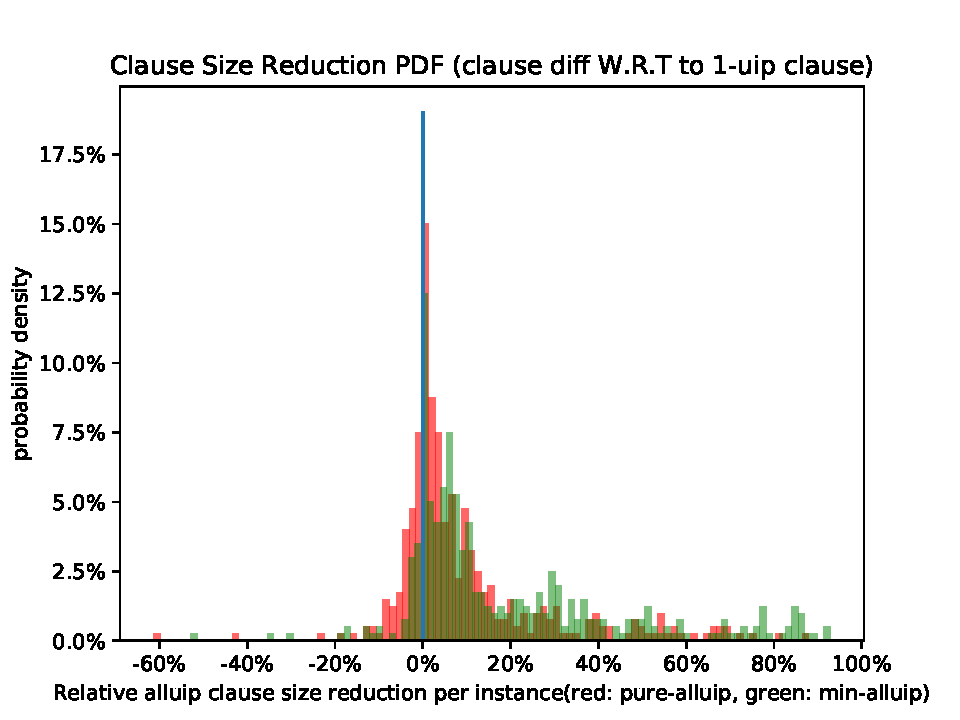
\includegraphics[width=\textwidth]{figures/clause_reduction_PDF.pdf}
   \caption{\fss{9pt}{10pt}
      Relative clause size reduction distribution. The $X$ axis
      indicates the relative size of difference between all-UIP and
      1-UIP clauses (calculated as
      $\dfrac{|C_1|-|C_i|}{|C_1|}$ ) for
      each instance, and the $Y$ axis shows the probability density.}
       \label{fig:len_pdf}
  \end{minipage}
  & &
  \begin{minipage}[t]{0.5\textwidth}
    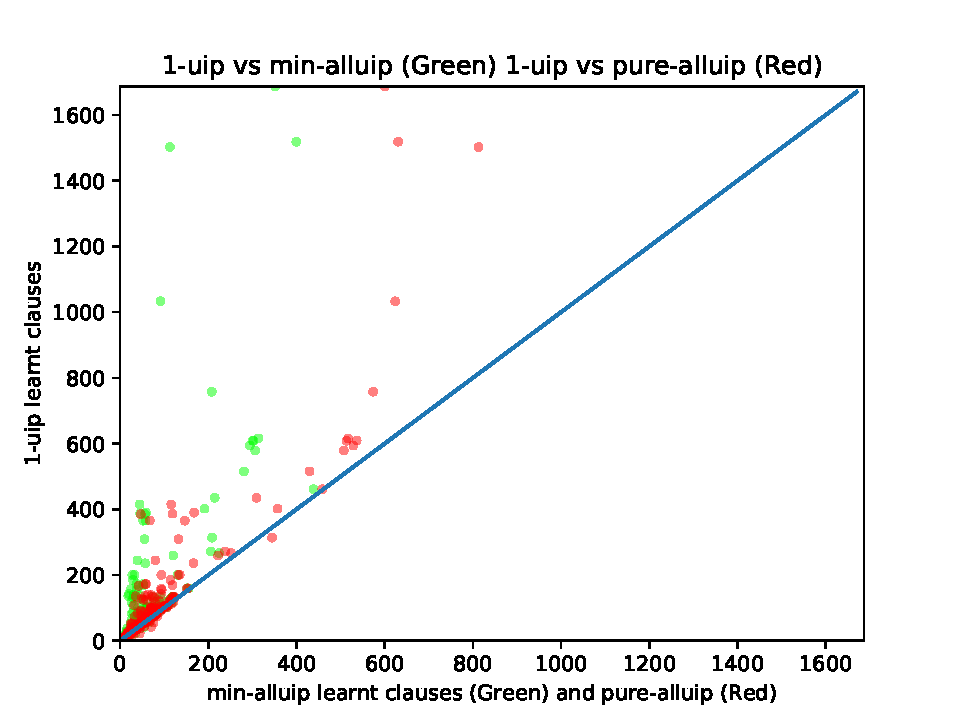
\includegraphics[width=\textwidth]{figures/clause_size_compare.pdf}
    \caption{\fss{9pt}{10pt}
      Average clause size comparison plot. Each point in the
      plot represents an instance. The $X$ and $Y$ axes shows the clause
      length from $\stablealluip$ and \oneuip, respectively. Each green (red)
      dot represents an compared instance between $\MapleBase$ and
      $\MapleIUIMin$ ($\allUipPure$).}
      \label{fig:len_compare}
  \end{minipage}
\end{tabular}
\end{figure}


\vspace*{3pt}\noindent\textbf{Reduced Proof Sizes with $\stablealluip$.}
A learning scheme that yields smaller clauses (lemmas) might also
construct smaller causal proofs. For 88 UNSAT instances solved mutually
by $\allUipPure$, $\allUipMin$ and \oneuip schemes, we additionally
compared the size of the optimized DRAT proof from the three learning schemes. 
We used the DRAT-trim tool
\cite{DBLP:conf/sat/WetzlerHH14} with a 30000 second timeout to check and
optimize every DRAT proof once\footnote{Applying DRAT-trim multiple
  times can further reduce the proof size until a fix-point. However,
  the full optimization is too time consuming for our
  experiments.}.

The average optimized DRAT proof from $\allUipMin$ and $\allUipPure$
are 556.6MB and 698.5MB, respectively. Both sizes are significantly
smaller than the average optimized proof size from \oneuip, 824.9MB.
The average proof size reduction per instance for $\allUipMin$ and
$\allUipPure$ is 16.5\% and 3.6\% against \oneuip, which roughly
correlate with our clause size observation in
Fig~\ref{fig:len_pdf}.

{  \setlength{\intextsep}{10pt}
\begin{figure} 
\begin{center}
\fss{9pt}{10pt}
\begin{tabular}{|l|l|l|l|} 
\hline
Solver & \#solved (SAT, UNSAT) $\Delta$ & PAR-2 & avg. clause Size \\ 
\hline
SAT 2017 Winner & & & \\
$\MapleSeven$ & 232 (135, 97) & 4755.96 & 61.9  \\ 
\hline
$\MapleSeven$-all-pure & \textbf{244 (146, 98)} +12 & \textbf{4504.18} & 43.76 \\
\hline
$\MapleSeven$-all-min & 240 (144, 96) +8 & 4601.25 & \textbf{36.97} \\ 
\hline
$\MapleSeven$-all-act & 237 (140, 97) +5 & 4678.434 & 43.62 \\ 
\hline
$\MapleSeven$-all-inclusive & 234 (137, 97) +2 & 4718.03 & 37.96 \\
\hline
\hline
SAT 2018 Winner & & & \\
$\MapleEightShort$ & 236 (138, 98) & 4671.81 & 61.69 \\
\hline
$\MapleEightShort$-all-pure & \textbf{241} (\textbf{142, 99}) +5 & \textbf{4598.18} & 44.19 \\
\hline
$\MapleEightShort$-all-min & 236 (141, 95) +0 & 4683.92 & 38.05 \\ 
\hline
$\MapleEightShort$-all-act & 240 (141, \textbf{99}) +4 & 4626.99 & 41.16 \\
\hline
$\MapleEightShort$-all-inclusive & 240 (\textbf{142}, 98) +4 & 4602.13 & \textbf{37.52} \\
\hline
\end{tabular}
\end{center}
\caption{Benchmark results of \oneuip, $\allUipPure$. $\allUipMin$, $\allUipAct$ and $\allUipIn$ on SAT2019 race main track instances.}
\label{fig:t5a}
\end{figure}
}

{ \setlength{\intextsep}{10pt}
  \setlength{\textfloatsep}{10pt}
\begin{figure} 
\begin{center}
\fss{9pt}{10pt}
\begin{tabular}{|l|l|l|l|} 
\hline
SAT 2019 Winner & & & \\
$\MapleNineShort$ & 238 (140, \textbf{98}) & 4531.24 & 60.91 \\
\hline
$\MapleNineShort$-all-pure & 240 (142, \textbf{98}) +2 & 4519.08 &  43.32\\
\hline
$\MapleNineShort$-all-min & 244 (\textbf{148}, 96) +6 & \textbf{4419.84} & \textbf{36.88} \\
\hline
$\MapleNineShort$-all-act & 243 (146, 97) + 5 & 4476.73 & 40.65 \\
\hline
$\MapleNineShort$-all-inclusive & \textbf{243} (\textbf{148}, 95) +5 & 4455.76 & 37.02 \\
\hline
\hline
SAT 2019 Competitor & & &\\
$\expSATShort$ & 237 (137, 100)  & 4628.96 & 63.19 \\
\hline
$\expSATShort$-all-pure & 235 (136, 99) $-$2  & 4668.96 & 48.26 \\
\hline
$\expSATShort$-all-min & 241 (143, 98) +4 & 4524.28 & 46.29 \\ 
\hline
$\expSATShort$-all-act & 244 (143, \textbf{101}) +7 & \textbf{4460.92} & 47.25 \\
\hline
$\expSATShort$-all-inclusive & \textbf{245} (\textbf{146}, 99) +8 & 4475.76 & \textbf{45.33}
\\
\hline
\hline
\cadical version 1.2.1 & & &\\
$\defaultcadical$ & 249 (150, 99)  & \textbf{4311.76} & 101.96 \\
\hline
$\defaultcadical$-all-pure & 248 (151, 97) $-$1  & 4373.38 & 82.44  \\
\hline
$\defaultcadical$-all-min & 248 (149, 99) $-$1 & 4398.31 & 43.93 \\ 
\hline
$\defaultcadical$-all-act & \textbf{252} (152, \textbf{100}) +3 & 4331.56 & 47.34 \\
\hline
$\defaultcadical$-all-inclusive & 251 (\textbf{153}, 98) +2 & 4335.88 & \textbf{42.61}
\\
\hline
\end{tabular}
\end{center}
\caption{Benchmark results of \oneuip, $\allUipPure$. $\allUipMin$, $\allUipAct$ and $\allUipIn$ on SAT2019 race main track instances.}
\label{fig:t5b}
\end{figure}
}

\begin{sloppypar}
    \vspace*{3pt}\noindent\textbf{$\stablealluip$ in Modern SAT
      solvers.}  To validate $\stablealluip$ in modern SAT solvers, we
    implemented $\stablealluip$ in the winners of 2017, 2018 and 2019
    SAT Race
    \cite{DBLP:conf/ijcai/LuoLXML17,ryvchin2018maple,Stepan2019MapleLCMDistChronoBT}
    and in the $\expSAT$ \cite{MdSolimul2019expMalpe} ($\expSATShort$)
    and $\cadical$~\cite{cadical} solvers. $\expSATShort$ is a top ten
    solver from 2019 SAT race which uses random walk simulation to
    help branching. We chose $\expSATShort$ because the random walk
    simulation branching heuristic is different from local branching
    heuristic (VSIDS and LRB) that we have considered in $\allUipAct$,
    $\allUipIn$, and $\allUipEx$. We chose $\cadical$ because its
    default configuration
%\footnote{$\cadical$'s default configuration is different from the specialized 'sat' configuration, which solved the most satisfiable instances in the 2019 SAT Race.} 
    ($\defaultcadical$) solved the most instances in the 2019 SAT Race
    (244). For this experiment, we used the latest available version
    of $\defaultcadical$ instead of the 2019 SAT Race
    version~\cite{Armin2019Cadical}.  We compared these solvers'
    base \oneuip learning scheme with $\allUipPure$, $\allUipMin$ and
    the top two $\stablealluip$ variants, $\allUipAct$ and
    $\allUipIn$, on the SAT Race 2019 main track benchmarks. We report
    solved instances, PAR-2 score and the average clause size.
\end{sloppypar}

Tables~\ref{fig:t5a} and \ref{fig:t5b} show the results of the
$\stablealluip$ configurations in our suite of modern
solvers. Overall, we observed similar performance gain on all modern
solvers as we have seen on $\MapleBase$ in Fig.~\ref{fig:t4}. More
specifically, almost all configurations improved on solved instance
(+3.9 instances in average) and PAR-2 score ($-$57.7 in average).  The
average clause size reduction is consistent across all solvers. Each
configuration also exhibits different strengths: $\allUipPure$ solved
the most instances with the best PAR-2 score on two solvers,
$\allUipMin$ yields small clauses, $\allUipIn$ solved the most SAT
instances, and $\allUipAct$ has stable performance.

On the SAT 2017 race winner $\MapleSeven$, all four configurations of
$\stablealluip$ solved more instances than \oneuip
learning. $\allUipPure$ solved more UNSAT and SAT instances while the
other configurations improved on solving SAT instances. The clause
size reduction of $\stablealluip$ is more significant on this solver
than on $\MapleBase$. The SAT 2018 race winner $\MapleEightShort$ uses
chronological backtracking (CB); three out of four configurations
outperformed \oneuip. On the SAT 2019 race winner $\MapleNineShort$,
all four $\stablealluip$ configurations solved more instances than
\oneuip. $\MapleNineShort$ prioritizes clauses that are learned
multiple times. We observed that $\stablealluip$ clauses are less
likely to be duplicated. As an example, $\allUipMin$ on average, added
12\% less duplicated clauses into the core clause database than
\oneuip. This observation is surprising, and the cause is unclear.

On $\expSATShort$, three out of four $\stablealluip$ configurations
solved more instances than \oneuip learning. We noticed that both
$\allUipAct$ and $\allUipIn$ show better performance than $\allUipMin$
and $\allUipPure$ on this solver. The random walk simulation branching
heuristic, however, didn't impact the performance of $\stablealluip$
schemes significantly.

$\defaultcadical$ with \oneuip solved 249 instances.  Applying
$\allUipAct$ and $\allUipIn$ helped the solver solve 3 and 2 more
instances, respectively.  The \oneuip clauses in $\defaultcadical$
were much larger than other solvers on average (101 vs 60) but the
$\stablealluip$ configurations yielded similar clause sizes.

\section{Conclusion}
In this paper we introduced a new clause learning scheme,
$\stablealluip$, that preserves the strengths \oneuip learning while
learning shorter clauses. We provided empirical evidence that using
$\stablealluip$ and its variants in modern CDCL solvers achieves
significant clause reduction and yields useful performance gains.

Our scheme extends \oneuip learning by performing further resolution
beyond the deepest decision level in an attempt to find the UIP at
each level in the learnt clause. Since resolutions may increase the
clause's \LBD by introducing literals from new decision levels, we
presented two methods to block such literals from entering the
clause. Although our learning scheme is conceptually simple, and we
presented optimizations to reduce and balance the learning cost. We
additionally presented variants of our schemes to account for features
used in state of the art solvers, e.g., local branching heuristics and
chronological backtracking.

Although the field of SAT solving has converged on using the \oneuip
learning scheme, we have shown the possibility of developing an
effective alternative through understanding the strengths and
weaknesses of \oneuip and clause learning schemes. Our learning scheme
can be generalized and further improved by exploring more fine-grained
trade-offs between different clause quality metrics beyond clause size
and \LBD. We also plan to study the interaction between clause
learning and variable branching. Since most of the branching
heuristics are tailored for \oneuip scheme, their interactions with
other learning schemes requires further study.

\bibliography{sat}{}
\bibliographystyle{splncs04}
\end{document}


